\chapter{Dataset}
\label{kap:dataset}
The main goal of machine learning is to gain the ability to generalize well on new, previously unseen data, in our case real-world images. This generalization is often only possible if the testing data comes from the same distribution as the training data. This distribution is sometimes difficult to obtain, especially in computer vision and computer graphics as we usually work with real-world imagery, for which is problematic to obtain ground-truth data. While we can collect depth and normals of a scene via depth sensors \cite{nyuv2}, it is complicated to generate data for albedo, lighting or other parameters.
\newline
This is where physically based rendering comes into play. When we render a scene following physically based techniques (thus, physically simulate light transportation in the scene), we can generate real-world like images for which we can obtain many properties of the rendered image, hence bridging the gap between synthetic datasets and real images.
\newline
Because of the lawsuit regarding SUNCG dataset we deciced to render our own dataset using PBR techniques to match the required image quality. Its scene complexity and richness of materials is unmatched by previously used datasets, which makes it superior for training. Some examples of images in our dataset are shown in figure \ref{fig:dataset-examples}.
\begin{figure}
  \centering
  \begin{subfigure}{0.4\linewidth}
    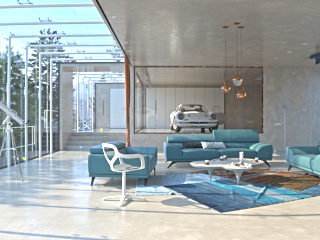
\includegraphics[width=\linewidth]{praca/images/Interior_mountain.png}
  \end{subfigure}
  \begin{subfigure}{0.4\linewidth}
    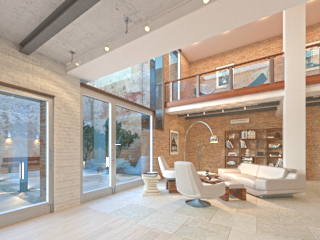
\includegraphics[width=\linewidth]{praca/images/AI50_001_Cam01.png}
  \end{subfigure}
  \begin{subfigure}{0.4\linewidth}
    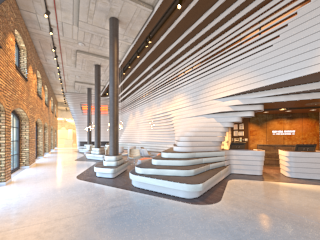
\includegraphics[width=\linewidth]{praca/images/AI44_006_Cam01.png}
  \end{subfigure}
  \begin{subfigure}{0.4\linewidth}
    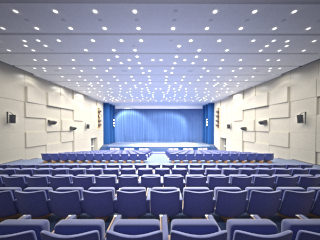
\includegraphics[width=\linewidth]{praca/images/AI53_005_Cam01.png}
  \end{subfigure}
  \caption[Examples of images in our dataset]{Examples of images in our dataset}
  \label{fig:dataset-examples}
\end{figure}
\newline
We started generating the dataset from $\approx$140 scenes downloaded from Evermotion website \cite{evermotion} by placing $\approx$10 virtual cameras inside every scene using 3ds Max \cite{3ds-max}. All images were rendered via V-Ray renderer \cite{V-Ray} from the viewports of those cameras to produce unique geometry for every camera view, with example in figure \ref{fig:camera-positions}.
\begin{figure}
  \centering
  \begin{subfigure}{0.4\linewidth}
    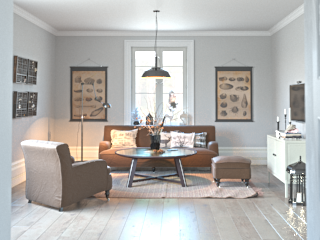
\includegraphics[width=\linewidth]{praca/images/AI43_008_Cam01.png}
  \end{subfigure}
  \begin{subfigure}{0.4\linewidth}
    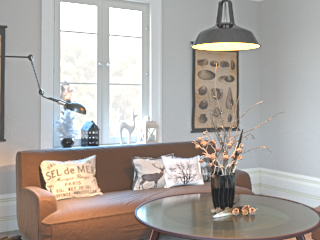
\includegraphics[width=\linewidth]{praca/images/AI43_008_Cam03.png}
  \end{subfigure}
  \begin{subfigure}{0.4\linewidth}
    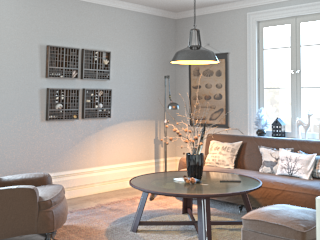
\includegraphics[width=\linewidth]{praca/images/AI43_008_Cam05.png}
  \end{subfigure}
  \begin{subfigure}{0.4\linewidth}
    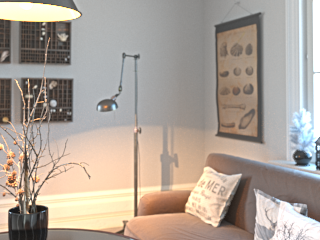
\includegraphics[width=\linewidth]{praca/images/AI43_008_Cam08.png}
  \end{subfigure}
  \caption[Different camera views for the same scene]{Different camera views for the same scene}
  \label{fig:camera-positions}
\end{figure}
\newline
To further enlarge the dataset, we make use of V-Ray's Light select feature \cite{V-Ray-Light-select} to turn on $\frac{1}{10}$ of lights presented in the scene, which generated up to 10 images of the same geometry under different lighting. As we found out during rendering, V-Ray optimizes computation for the main image, which has most of the lights turned on. When only a subset of lights is turned on for light select element, rendered image can be quite noisy, or due to poor selection of the lights, it can even be full black image. In scenes where this approach did not work and rendered light select images were noisy, we had to do it the other way around - we turned on $\frac{9}{10}$ of all lights in the scene. Combination of these two approaches generated 5-7 different lighting conditions for most of the scenes. Examples of mentioned light alternations are shown in figure \ref{fig:light-alternations}.
\begin{figure}
  \centering
  \begin{subfigure}{0.4\linewidth}
    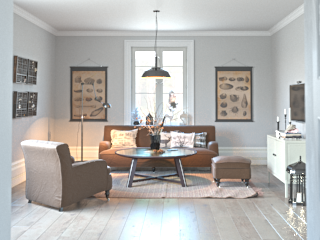
\includegraphics[width=\linewidth]{praca/images/AI43_008_Cam01.png}
  \end{subfigure}
  \begin{subfigure}{0.4\linewidth}
    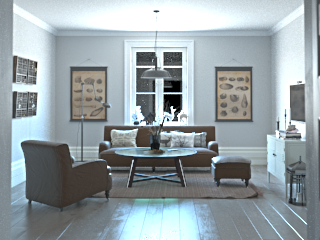
\includegraphics[width=\linewidth]{praca/images/AI43_008_Cam01.VRayLightSelect_RE_L0.png}
  \end{subfigure}
  \begin{subfigure}{0.4\linewidth}
    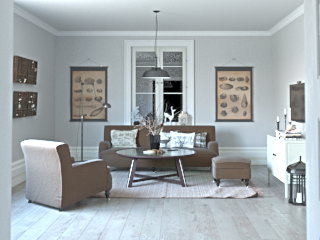
\includegraphics[width=\linewidth]{praca/images/AI43_008_Cam01.VRayLightSelect_RE_L1.png}
  \end{subfigure}
  \begin{subfigure}{0.4\linewidth}
    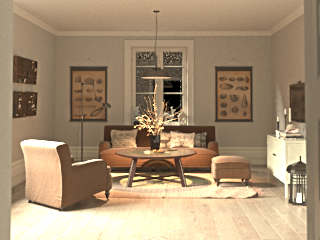
\includegraphics[width=\linewidth]{praca/images/AI43_008_Cam01.VRayLightSelect_RE_L4.png}
  \end{subfigure}
  \caption[Different lighting for the same camera view]{Different lighting for the same camera view}
  \label{fig:light-alternations}
\end{figure}
\noindent As we decided to choose similar approach as showed in \cite{sengupta-inverse-rendering}, we also had to include environment maps into our dataset. To ensure that we had enough maps for training, we opted for combination of publicly available HDRI maps on HDRI Haven website \cite{hdri-haven} - with 105 maps - and our own dataset of environment maps by generating 360$^{\circ}$ panoramas of size $18 \times 36$ pixels for every scene, yielding 1005 maps. In total, we have about $5\times$ more environment maps than was used in \cite{sengupta-inverse-rendering}.
\newline
All of the rendering was done on powerful 30 core CPU machines. Altogether, the dataset took about 1000 hours to render. Some scenes took very long to render, so we also tried rendering on GPU, but for some unknown reason we were not able to match the same image quality. If we want to render larger dataset in the future, we will have to find a way to fix the setup for GPU rendering, as it presents great promises in reducing rendering time.
\newline
In the end, our dataset consists of 1041 unique scene geometries, 1110 environment maps and 5709 images in total under different lighting conditions with ground-truth data like diffuse albedo, specular albedo, normals, depth, glossiness and view vector obtained as render elements feature of V-Ray \cite{V-Ray-Render-elements}. V-Ray provides also a render element containing index of a directly visible material for every pixel which we used to create ground-truth data for material segmentation. We modified output of the original render element by replacing each index by an RGB color computed by taking the most frequent diffuse albedo $\rho^*_d$ and specular albedo $\rho^*_s$ in all pixels with the same index and combining them using formula:
$$\frac{\rho^*_d + \rho^*_s}{2}$$
In our testing, we found this to work well in assigning different colors to different materials and not overlap too much. One problem, however, arises. For now, we do not have to know the values of diffuse and specular albedo that made the final pixel value in the segmented image. If we wanted to get those values (for example, to adjust values predicted by neural net), we would have to choose an invertible coding. In figure \ref{fig:dataset-gt}, you can see example of ground-truth data for one scene.
\newline
As V-Ray supports more than 60 render elements, our dataset is easily extendable with new characteristics of a scene for additional work in the future.
\begin{figure}
  \centering
  \begin{subfigure}{0.3\linewidth}
    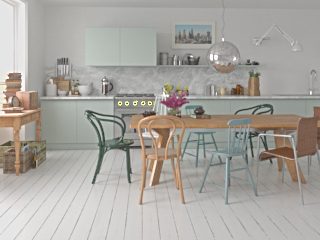
\includegraphics[width=\linewidth]{praca/images/AI43_001_Cam01.png}
    \caption{Main Image}
  \end{subfigure}
  \begin{subfigure}{0.3\linewidth}
    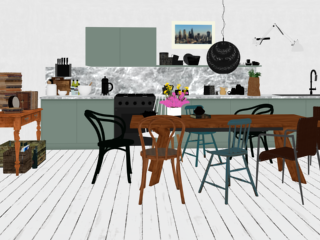
\includegraphics[width=\linewidth]{praca/images/AI43_001_Cam01.VRayRawDiffuseFilter.png}
    \caption{Diffuse Albedo}
  \end{subfigure}
  \begin{subfigure}{0.3\linewidth}
    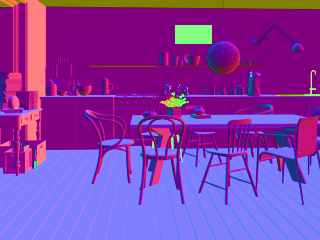
\includegraphics[width=\linewidth]{praca/images/AI43_001_Cam01.VRaySamplerInfoNormal.png}
    \caption{Normals}
  \end{subfigure}
  \begin{subfigure}{0.3\linewidth}
    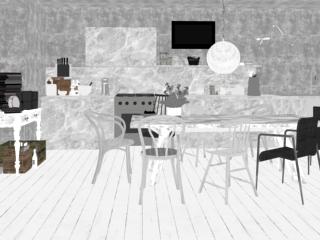
\includegraphics[width=\linewidth]{praca/images/AI43_001_Cam01.VRayRawReflectionFilter.png}
    \caption{Specular Albedo}
  \end{subfigure}
  \begin{subfigure}{0.3\linewidth}
    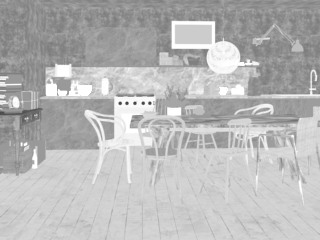
\includegraphics[width=\linewidth]{praca/images/AI43_001_Cam01.VRayMtlReflectGlossiness.png}
    \caption{Glossiness}
  \end{subfigure}
  \begin{subfigure}{0.3\linewidth}
    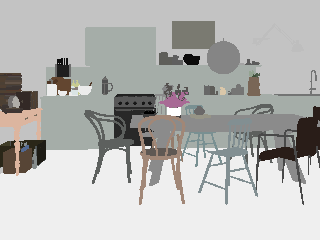
\includegraphics[width=\linewidth]{praca/images/AI43_001_Cam01.VRayMtlID.png}
    \caption{Material Segmentation}
  \end{subfigure}
  \begin{subfigure}{0.3\linewidth}
    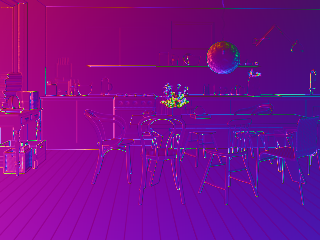
\includegraphics[width=\linewidth]{praca/images/AI43_001_Cam01.VRaySamplerInfoView.png}
    \caption{View vector}
  \end{subfigure}
  \begin{subfigure}{0.3\linewidth}
    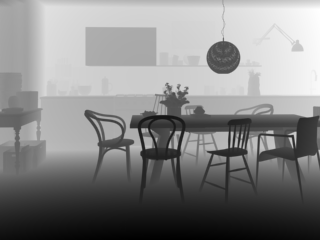
\includegraphics[width=\linewidth]{praca/images/AI43_001_Cam01.VRayZDepth.png}
    \caption{Depth}
  \end{subfigure}
  \begin{subfigure}{0.3\linewidth}
    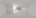
\includegraphics[width=\linewidth]{praca/images/AI43_001_Cam01.360.png}
    \caption{Env Map}
  \end{subfigure}
  \caption[Example of GT data for a scene]{Example of ground-truth data for a scene}
  \label{fig:dataset-gt}
\end{figure}